
% Desc: Stage user manual
% Author: Richard Vaughan, Andrew Howard
% Date: 10 Jun 2002
% CVS: $Id: stage.tex,v 1.5 2002-11-11 08:21:39 rtv Exp $

\documentclass[11pt,twoside]{report}

% this one apparently fixes the < and > chars
\usepackage[T1]{fontenc}
\usepackage{subfigure}
\usepackage{times}
\usepackage{tabularx}

% why did we need this?
%\usepackage{verbatim}
% make all captions small and slanted
\usepackage[small,sl]{caption}
\usepackage{fullpage}
%\usepackage{epsf}
\usepackage{epsfig}
\usepackage{graphicx}
% add nifty DRAFT watermark thingy in PS
%\usepackage{draftcopy}

% A nice environment for displaying command line args (AH)
\newenvironment{xarg}[1]{\noindent{\tt #1}\\\hspace*{2em}\begin{minipage}[t]{5in}}{\end{minipage}\vspace*{1em}}

\def\VERSION {1.3}
\def\HOMEPAGE {{\tt http://playerstage.sourceforge.net}}
\def\SFPAGE {{\tt http://sourceforge.net/projects/playerstage/}}

\begin{document}

\setcounter{page}{0}
\pagenumbering{roman}

\titlepage

 \begin{tabular}{lcr}
   \begin{tabular}{c}
 	Player/Stage project\\
         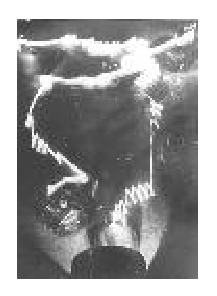
\includegraphics{notext_ps_logo}
    \end{tabular}
   &
   \hspace{5cm}
   &
   \begin{tabular}{r}
     {\bf USC Robotics Laboratory}\\
     University of Southern California\\
     Los Angeles, California, USA\\
     \vspace*{2em}\\
     {\bf Information Sciences Laboratory}\\
     HRL Laboratories\\
     Malibu, California, USA\\
   \end{tabular}
 \end{tabular}


  \vspace{5cm}	
  \centerline{ \Huge{Stage}}
  \vspace{0.5cm}
  \centerline{\large{Version \VERSION\ User Manual}}
  \vspace{2cm}
  \centerline{\large Richard T.~Vaughan \\ Andrew Howard \\ Brian P.~Gerkey}
  \vspace{1cm}

  \centerline{This document may not contain the most current documentation on}
  \centerline{Stage.  For the latest documentation, consult the Player/Stage homepage:}
  \centerline{\HOMEPAGE}

  \vspace{4cm}

 \centerline{\today}

\tableofcontents
%\newpage

%\listoffigures
%\newpage
%\listoftables
%\newpage

% reset page number to start with 1
\setcounter{page}{0}
\pagenumbering{arabic}


\chapter{Introduction}

  \section{What is Stage?}

    Stage is a product of the Player/Stage Project, a collection of
    software tools to support research in autonomous robotics and
    intelligent sensor systems.  Stage simulates a population of
    mobile robots, sensors and objects in a two-dimensional bitmapped
    environment. Stage is designed with multi-agent systems in mind,
    so it provides fairly simple, computationally cheap models of lots
    of devices rather than attempting to emulate any device with great
    fidelity. We have found this to be a useful approach.

    Stage devices are usually controlled through \emph{Player}; a
    networked robot server. Player provides a convenient interface to
    a set of device drivers for real robots and sensors. Stage
    simulates a population of devices and makes them available thorugh
    Player. Users
    write robot controllers and sensor algorithms as `clients' to the
    Player `server'. Typically, clients cannot tell the difference
    between the real robot devices and their simulated Stage
    equivalents (unless they try very hard). We have found that
    clients developed using Stage will work with little or no
    modification with the real robots and vice versa. Thus Stage
    allows rapid prototyping of controllers destined for real
    robots. Stage also allows experiments with realistic robot devices
    you don't happen to have.
  
    Various sensors and actuators are provided, including sonar,
    scanning laser rangefinder, color-blob vision, odometry, grippers,
    bumpers/whiskers and mobile robot bases.

  \section{How to get Stage and related software}

   The main resource for Player/Stage is the project
    homepage:\\\\ \indent \HOMEPAGE\\
	
   \noindent Access to source code releases, access to the CVS
   development tree, bug tracking, user mailing lists, etc.~ is
   available from the Sourceforge project management page:\\\\\indent
   \SFPAGE\\

   \noindent The current release is available as the source tarball
 Stage-<version>.src.tgz at:\\\\ \indent
 http://sourceforge.net/project/showfiles.php?group\_id=42445\\

	Previous versions were significantly different; this manual
   does not apply to them.

  \section{What's in the Package?}

    In the release tarball you will find:
      \begin{itemize}    
      \item C++ source code for 'stage' the simulation engine.
      \item Example environments and setup files.
      \end{itemize}



  \section{Requirements}

    \begin{itemize}
    \item Player [\HOMEPAGE]
    \item libstdc++
    \end{itemize}
    
    Optional (but highly recommended): 
    \begin{itemize}
      \item libRTK [\HOMEPAGE]
	\begin{itemize}
	  \item X11R6, GTK++.
\end{itemize}
	\end{itemize}

    Stage was developed and tested under Linux kernel 2.4,
    glibc-2.2.  Code is reasonable ANSII/POSIX so it should compile
    elsewhere. No promises, but people have found it to work on a
    variety of set-ups.
  
  \section{Ownership}

    Stage is released under the GNU General Public
    License. Stage programs, images, examples, source code and
    documentation are copyrighted by their their authors. The authors are:

      \begin{itemize}
      \item[] Richard Vaughan [rtv@sourceforge.net]
      \item[] Andrew Howard [inspectorg@sourceforge.net]
      \item[] Brian Gerkey [gerkey@sourceforge.net]
      \item[] Kasper Stoy [kaspers@robotics.usc.edu]
      \item[] Boyoon Jung [boyoon@robotics.usc.edu]
      \item[] Jakob Fredslund [jakobf@robotics.usc.edu]
      \end{itemize}

	See your name here by contributing devices, superior
	algorithms, bugfixes, examples, etc.

  \section{Bugs and feedback}
  
    This is constantly evolving research software. It is bound to
    contain bugs, despite developer and user testing.  If you find
    something that appears to be a bug, or if some aspect of Stage's
    behavior seems wrong or non-intuitive, let us know. If you have a
    problem, please check the website and bug tracking logs. If you
    can't find an answer there, use the bug tracker to tell us about
    the problem. Better still, fix it and send us the patch. To stay
    in touch with the developers and other users, join the mailing
    lists.

    When submitting bugs, include as much information as possible,
    including the Stage version, OS type and version, and any output
    messages.  A detailed description of what happened will enable us
    (hopefully) to repeat and analyze the problem.  Of course, there
    is NO WARRANTY on this software, and no guarantee that we will fix
    your problem.  But we use Stage for our research and we want it to
    work properly, so we will do our best. Again {\emph please use the
    sourceforge bug tracking tools}; that's the best way to see your
    problem solved.

  \section{What happened to...?}
	
	Previous releases contained some supplementary programs which
	have been removed during development of
	Stage-\VERSION. 'RTKStage' has been folded into Stage. Stage
	client mode makes 'XS' redundant. Stage server makes 'manager'
	redundant. Don't worry; things are better now.

\section{Citations}
If you find Player and Stage useful in your work, we would greatly
appreciate your mentioning that fact in papers that you publish.  A
paper of our own on Player has been presented in a respected
peer-reviewed conference; this paper is the definitive reference when
citing Player \cite{GerkeyVaughan01a}:
\begin{quote}
Brian~P. Gerkey, Richard~T. Vaughan, Kasper St\o{}y, Andrew Howard,
Maja~J Matari\'c and Gaurav~S Sukhatme.
\newblock {Most Valuable Player: A Robot Device Server for Distributed
  Control}.
\newblock In {\em Proc. of the IEEE/RSJ Intl. Conf. on Intelligent Robots and
  Systems (IROS)}, pages 1226--1231, Wailea, Hawaii, October 2001.
\end{quote}

At the time of writing, there is no peer-reviewed article about Stage,
but there is a USC technical report, available at:

\begin{quote}
Richard T.~Vaughan. "Stage: A Multiple Robot Simulator". Technical Report IRIS-00-394, Institute for Robotics and Intelligent Systems, School of Engineering, University of Southern California, 2000.
\end{quote}

These papers (and any new ones) are available at: 

\begin{verbatim}
   http://playerstage.sourceforge.net/pubs.html
\end{verbatim}

If you have space (and are feeling generous), you can also insert a footnote
similar to the following:
\begin{quote}
Player and Stage were developed jointly at the USC Robotics Research
Lab and HRL Labs and are freely available under the GNU General Public
License from http://playerstage.sourceforge.net.
\end{quote}
By including such acknowledgements, you do more than feed our egos and
further our careers.  You spread the word about the Player/Stage
project, which will bring more users and developers, as well as please
our funders, ensuring that we will continue hacking on the software.

  \section{Acknowledgements}

Stage originated at the University of Southern California Robotics
    Labs. Support at USC has come from DARPA grant DABT63-99-1-0015
    (MARS), NSF grant ANI-9979457 (SCOWR), DARPA contract
    DAAE07-98-C-L028 (TMR), ONR Grants N00014-00-1-0140 and
    N0014-99-1-0162, and JPL Contract No. 1216961. Development at HRL
    Laboratories is supported by a DARPA contract (SDR). Thanks to
    Doug Gage at DARP IPTO.

Thanks to our contributors and users, particularly the USC Robotics
Lab students and alumni who have been generous with their advice, bug
fixes, and contributions. These fine people have contributed code:
Esben \O{}sterg\aa{}rd, Jakob Fredslund, Boyoon Jung, Jason
K. Douglas, Kim Jinsuck, Gabe Sibley, and Dave Naffin. Contributed
tools can be found on the website.

%////////////////////////////////////////////////////////////////////////////
\chapter{Running Stage}
  \section{Building and Installing Stage}

  You must install Player {\em before} building Stage. To build Stage
 with an interactive GUI, which is highly recommended, you must
 install libRTK before building Stage. Player and libRTK are availabe
 from the Player/Stage files page:
	\begin{verbatim}
	http://sourceforge.net/project/showfiles.php?group_id=42445
	\end{verbatim}
	\noindent Build and install Player and libRTK following the
	instructions in the packages' README and INSTALL files. Now
	download thew Stage tarball and unpack it with:
      \begin{verbatim}
      $ tar xzvf Stage-1.2.tgz
      \end{verbatim}
   \noindent Now follow the instructions for your release in the
    top-level README and INSTALL files.

  \section{Running Stage}

    Before running stage, first make sure the Player executable can be
    found in your path (Stage will automatically start an instance of
    Player, so it needs to know where to find the Player executable).
    For example, try:
      \begin{verbatim}
      $ which player
      \end{verbatim}
    and make sure it returns a valid Player executable path, such as
      \begin{verbatim}
      ~/player-1.3/bin/player
      \end{verbatim}
    If not, set your PATH variable to include the Player binary directory. 
    For example, in BASH do:
      \begin{verbatim}  
      $ export PATH=$PATH:$HOME/player-1.2/bin
      \end{verbatim}  

    The general command line to run Stage is: 
      \begin{verbatim} 
      stage [options] <filename.world> 
      \end{verbatim} 

    By convention, Stage configuration files end with a `.world'
    extension and are referred to as 'world files'. A world file
    specifies what stage must simulate. The user can override some of
    the world file settings at run time using the command-line options
    described below. If all is well, Stage will start up, load the
    world file, and spawn an Player. Each step causes a message on
    standard output, so a sample invocation and start up would look
    like this:

	\begin{verbatim} 
	$ stage worlds/everything.world

	 ** Stage  v1.3 ** 
	[World worlds/everything.world]
	[Server localhost:6601]
	** Player v1.3 ** [Stage /tmp/stageIO.username.0]
      \end{verbatim}

    At this point you should be able to interact with objects in the
    world with the GUI (try dragging things around) and access sensors
    and actuators through Player. Try using the Player client program
    (<player\_root>/utils/playerv/playerv) to see the output from some
    sensors.

    %Should probably have a Help! It didnt work section. AH
    %If it didn't work, the first things to check are the
    %settings in Makefile.common and your Player build.
  
  \section{The World File}

    The world file is a description of the world that Stage must
    simulate.  It describes robots, sensors, actuators, moveable and
    immovable objects.  The world file can also be used to control
    many aspects of the simulation engine, such as its speed and
    fidelity.  See Chapter \ref{sec:world} for a complete description
    of the world file format.  Sample world files can also be found in
    the `worlds' directory.

  \section{Command Line Arguments}

    Stage takes the following command-line options. Where an option
    can also be set in the configuration file, the command line option
    takes precedence.

    \begin{xarg}{-n} No Player - do not spawn a Player. You can run
    Player manually in Stage mode with
    \verb+player -stage <device dir>+. Useful for debugging Player or
    if you want to use an alternative interface to Stage
    devices.
    \end{xarg}

    \begin{xarg}{-g}Disables the Graphical User Interface.
    \end{xarg}

    \begin{xarg}{-o}Output mode - enables console output showing
    timing and data throughput information \end{xarg}

    \begin{xarg}{-t <timeout in seconds>}Timeout - Stage will quit
    after simulating the specified amount of time. Useful for batch
    runs.  
    \end{xarg}

    \begin{xarg}{-u <update period in seconds>}
    Stage will attempt to take this much real time (wall-clock time)
    to perform each update cycle. It does this by computing the cycle,
    then sleeping (or polling for input) for any remaining time. If
    the cycle's computation takes longer than the requested cycle
    time, Stage will run slower than requested. Default is 0.1
    seconds.
    \end{xarg}

    \begin{xarg}{-v <simulation time step in seconds>}
    Stage will simulate the passing of this much time per update
    cycle. Default is 0.1 seconds. By changing the ratio of real (-u)
    and simulated (-v) time, you can make Stage run faster than,
    slower than, or approximately at real-time.
    \end{xarg}

    \begin{xarg}{-f} Fast mode - Stage will run as fast as possible;
    not attempting to match real time. Useful for batch runs. This is
    slightly more efficient than setting the desired update time to
    zero seconds (-u 0.0).  
    \end{xarg}

    \begin{xarg}{-s} Stopped - Stage will start up with the clock stopped.
      You can start and stop the clock by sending Stage a SIGUSR1 signal
      (\verb'killall -s USR1 stage' should do the trick; this command is
      provided as the script <stage\_root>/tools/pause.).
    \end{xarg}


%% RTV - ommitting client/server stuff for 1.3
%%     \begin{xarg}{-c <hostname>}Client mode - run Stage as a client to
%%     a Stage server on <hostname>. See below for discussion of Stage
%%     client/server.  \end{xarg}

%%     \begin{xarg}{-cl}Client mode, server on localhost - equivalent to '-c localhost' 
%% 	 \end{xarg}

%%     \begin{xarg}{-p <port num>}
%%     Set the port number for the Stage server to accept connections. Default is 6601.
%%     \end{xarg}

%%    \begin{xarg}{-l <logfile>} Enables logging of timing and
%%   throughput measurements into <logfile>.<incrementing counter>. The
%%  file has a header that records information about the run, and
%%    explains the format.
%%    \end{xarg}

\section{Controlling the robots}

The virtual robots in Stage are controlled through the Player.  Demo
controllers in various languages (currently C++, C, TCL \& LISP) are
included in the Player distribution.

Try using the Player example client
\verb+<player_root>/utils/playerv/playerv+ to check that you can control
Stage robots and read from their sensors. playerv is a very useful
tool for testing and debugging your controller code.

Client libraries in other languages including Java and Python are also
available. Check the website for the latest resources.

\section{Starting and Stopping the clock}

Stage's internal clock can be started and stopped by sending Stage a
SIGUSR1, for example with the command:
\begin{verbatim}
killall -s USR1 stage
\end{verbatim}.
The script \verb'<stage_root>/tools/pause' executes this command.

%% \section{Stage Server and Clients}
%% Internally, Stage consists of an environment and a collection of
%% devices. Together these comprise a world model. Stage also contains a
%% GUI which shows the state of the world and allows the user to
%% manipulate objects. This is all that many users need to use. However,
%% Stage also contains a network server that allows external client
%% programs to obtain complete information about the world. Eventually,
%% Stage will be capable of distributing compute load across multiple
%% clients (``imagine a Beowulf cluster of those'', etc.). For now, Stage can
%% act as a client to itself. This is great as an external networked
%% viewer (it replaces the old program XS). For example, you can run
%% Stage on one machine without a gui:

%% \begin{verbatim}
%% batman% stage -g examples/everything.world 
%% \end{verbatim}

%% It'll start up and run as normal (actually a little faster than normal
%% as it isn't working on the GUI). When you want to see what's going on, you can start up another Stage in client mode:

%% \begin{verbatim}
%% batman% stage -c localhost
%% \end{verbatim}

%% or equivalently, use the '-cl' client-to-localhost option:

%% \begin{verbatim}
%% batman% stage -cl
%% \end{verbatim}

%% The Stage client should start up, connect to the Stage server running
%% on the local machine, download the world and allow you to interact
%% with it as normal. When you're done, you can quit the client; the
%% server keeps running. Even better, you can run the Stage client on a
%% different machine and connect via the network to the server:

%% \begin{verbatim}
%% robin% stage -c batman
%% \end{verbatim}

%% Stage can handle many simultaneous clients.

%////////////////////////////////////////////////////////////////////////////
\chapter{Using the Stage GUI}

Stage presents a single conventional resizable window with a menu and
a main display area showing a view of the world.

\section{World view}
The main display area shows the world, the simulated entities (objects
and devices), and optionally, representations of the data generated
by devices. 

\subsection{Mouse}
The user can pan and zoom the world view and manipulate entities with
the mouse:

\subsubsection*{Clicks on the background}

\begin{tabular}{|l|l|}
\hline Mouse action & Result\\\hline
Left-click and drag & pan the window\\
Right-click and drag TOWARDS the center of the window & zoom in\\
Right-click and drag AWAY FROM the center of the window & zoom out\\ 
\hline
\end{tabular}

\subsubsection*{Clicks on entities}
\begin{tabular}{|l|l|}
\hline Mouse action & Result\\\hline
Left-click and drag & move the entity\\
Right-click and drag & rotate the entity\\
\hline
\end{tabular}

\subsection{Keyboard}
The world view can also be panned and zoomed with the keyboard. The
keybindings are:

\subsubsection*{Clicks on entities}
\begin{tabular}{|l|l|}
\hline Key & Action\\ \hline
<arrowkeys>        & scroll the window \\
<ctrl><arrowkeys>  & scroll the window in large increments \\
<shift><uparrow>   & zoom in \\
<shift><downarrow> & zoom out \\
\hline 
\end{tabular}

\section{Menu}

\subsection{File Menu}

\begin{tabular}{|l|l|}
\hline 
Save & save current world state into worldfile\\
Export & export a picture of world state as an xfig file (needs work)\\
Quit & exit Stage\\
\hline
\end{tabular}

\subsection{View Menu}

\begin{tabular}{|l|l|}
\hline 
Grid & toggle view of a 1m grid\\
Matrix & toggle view of underlying bitmap representation\\
Data menu & toggle visualizations of data generated by devices\\
Object menu & toggle visualizations of object bodies\\
\hline
\end{tabular}

\subsection{Action Menu}

\begin{tabular}{|l|l|}
\hline 
Subscribe to all & toggle Player subscriptions to all devices,
enabling data visualization for just about evetrything. \\
\hline
\end{tabular}


%////////////////////////////////////////////////////////////////////////////
\chapter{The World File}
\label{sec:world}

The world file is used to describe the particular set of robots,
sensors and objects to be simulated by Stage.  Stage reads the world
file on start-up and creates entities as indicated in the file.  Stage
may also write updated pose information into the world file when the
user selects the {\bf File:Save} menu option.

Note that the world file format has changed significantly from
previous versions. The script \verb+tools/worldfileconv.tcl+ will
attempt to convert your old (pre Stage-1.2) world files to the new
format.

\section{Basic Syntax}

A simple world file might look like this:
\begin{quote}
\begin{verbatim}
# This world file creates two robots with lasers.

environment 
( 
  file "cave.pnm" 
  scale 0.03 
)

position 
( 
  name "robot1" port 6665 pose [1 1 0] 
  player ()
  laser ()
)

position 
( 
  name "robot2" port 6666 pose [2 1 0] 
  player ()
  laser ()
)
\end{verbatim}
\end{quote}
This example shows the basic syntactic features of the 
world file format: comments, entities and properties.
%
Comments are indicated by the \verb'#' symbol; they may be placed
anywhere in the file and continue to the end of the line.  For
example:
\begin{quote}
\begin{verbatim}
# This world file creates two robots with lasers.
\end{verbatim}
\end{quote}
%
Entities are indicated using \verb'type ( ... )' entries; each such
entry instantiates an entity of type \verb'type'.  For example:
\begin{quote}
\begin{verbatim}
position ( ... )
\end{verbatim}
\end{quote}
creates a single position device (a bare-bones mobile robot).  Entities may
be nested to indicate that one entity is a ``child'' of another; thus:
\begin{quote}
\begin{verbatim}
position ( player () laser() )
\end{verbatim}
\end{quote}
creates a single position device with a Player server and laser attached to
it.  Think of child entities as physically sitting on their parent.
%
Entities have properties, indicated using \verb'name value' pairs:
\begin{quote}
\begin{verbatim}
position ( name "robot1" port 6665 pose [1 1 0] ... )
\end{verbatim}
\end{quote}
This entry creates a position device named ``robot1'' attached to port
6665, with initial position $(1, 1)$ and orientation of $0$.  Property
values can be either numbers (\verb'6665'), strings (indicated by
double quotes \verb'"robot1"') or tuples (indicated by brackets
\verb'[1 1 0]'). 

\section{Defining new entity types}

The \verb'define' statement can be used to define new types of entities.
For example, the world file from the previous section can be re-written
in a more concise form as follows:
\begin{quote}
\begin{verbatim}
# This world file creates two robots with lasers.
# It uses the 'define' construct to define a new type of entity.

environment ( file "cave.pnm" scale 0.03 )

define myrobot position ( player() laser() )

myrobot ( name "robot1" port 6665 pose [1 1 0] )
myrobot ( name "robot2" port 6666 pose [2 1 0] )
\end{verbatim}
\end{quote}
New entities are defined using \verb'define newentity oldentity (...)'.
For example, the line:
\begin{quote}
\begin{verbatim}
define myrobot position ( player() laser() )
\end{verbatim}
\end{quote}
defines a new \verb'myrobot' entity type composed of the
primitive \verb'position', \verb'player' and \verb'laser' entities.
This entity may be instantiated using the standard syntax:
\begin{quote}
\begin{verbatim}
myrobot ( name "robot1" port 6665 pose [1 1 0] )
\end{verbatim}
\end{quote}
This entry creates a position device named \verb'robot1' that has
both \verb'player' and \verb'laser' devices attached.

\section{Using include files}

The \verb'include' statement can be used to include entity definitions
into a world file.  For example, the world file from the previous section
can be divided into an include file called \verb'myrobots.inc':
\begin{quote}
\begin{verbatim}
# This is an include file.
# It uses the 'define' construct to define a new type of entity.

define myrobot position ( player() laser() )
\end{verbatim}
\end{quote}
and a world file called \verb'myworld.world':
\begin{quote}
\begin{verbatim}
# This world file creates two robots with lasers.
# It uses the 'include' statement to include the robot definitions.

include "myrobots.inc"

environment ( file "cave.pnm" scale 0.03 )

myrobot ( name "robot1" port 6665 pose [1 1 0] )
myrobot ( name "robot2" port 6666 pose [2 1 0] )
\end{verbatim}
\end{quote}
The definitions are included using the \verb'include "filename"'
statement.

\section{Units}

The default units for length and angles are meters and degrees
respectively.  Units may be changed using the following global
properties:
\begin{table}[h]
\begin{tabularx}{\columnwidth}{llX}
\hline
Name & Values & Description \\
\hline

\verb'unit_length' & \parbox{30mm}{\verb'"m"'\\\verb'"cm"'\\\verb'"mm"'}
& Set the unit length to meters, centimeters or millimeters. \\

\verb'unit_angle' & \parbox{30mm}{\verb'"degrees"' \\ \verb'"radians"'} &
Set the unit angle to degrees or radians.\\

\hline
\end{tabularx}
\end{table}

\noindent The following example uses millimeters rather than meters
for the unit length unit:
\begin{quote}
\begin{verbatim}
# This world file creates two robots with lasers.
# It uses the 'include' statement to include the robot definitions.

unit_length "mm"

include "myrobots.inc"

environment ( file "cave.pnm" scale 30 )

myrobot ( name "robot1" port 6665 pose [1000 1000 0] )
myrobot ( name "robot2" port 6666 pose [2000 1000 0] )
\end{verbatim}
\end{quote}
Be warned that the length specfication applies to the include files as well,
so choose a unit length early and stick to it.


\section{Examples}

See the {\tt examples} directory in the Stage distribution for more
world file examples.


\chapter{Entity Reference}

This chapter describes all of the models supported by Stage.  All
entity types defined in the world file are ultimately composed of one
or more models. Each model is implemented by code in
<stage\_src>/src/models.


\section{Properties and the type heirarchy}

Each model has zero or more {\em properties} associated with it; these
properties specify characteristics such as an object's shape or a
sensor's range.  Models are organized into a heriarchy, with sub-types
inheriting properties from their parent type.  All passive
environmental objects (boxes, pucks and bitmaps) are derived from a
basic \verb'entity' type and are referred to as \em{objects}.
Similary, all sensors and actuator models are derived from a generic
\verb'device' type, and referred to as \em{devices}. The \verb'device'
type is itself derived from \verb'entity', so they devices inherit all
the standrd entity properties. 

Note that both the \verb'entity' and \verb'device' types are {\em
abstract} (in C++ parlance) since they cannot be instantiated
directly.

%\newpage
\section{Object Summary}
\label{sec.ref.objects}

The following table lists all of the {\em objects} (models of passive
environmental objects) supported by Stage. They are described in
detail in the following pages. See Section \ref{sec.ref.devices} for a
list of Stage's {\em devices}.
\vspace{1em}\\\noindent
\begin{tabularx}{\columnwidth}{llX}
\hline 
Type & Parent type & Description \\
\hline 


\verb'entity' & None & A generic entity, which has shape, exent and
color - cannot be instantiated directly. \\

\hline

\verb'bitmap' & \verb'entity' & A pattern of fixed obstacles loaded
from a PNM bitmap file. Used to import building floorplans, walls,
boulders, etc. \\

\verb'box' & \verb'entity' & A fixed obstacle (can be moved by the
user but not the robot). \\

\verb'puck' & \verb'entity' & A movable object (can be moved by both
the user and the robot).\\

\hline
\end{tabularx}
\vspace{1em}\\



\newpage
\subsection{The {\tt entity} base type}

\subsubsection*{Parent}
{\tt <none>}

\subsubsection*{Description}
All Stage models are derived from the generic \verb'entity' type.
While this type can not be instantiated directly, all descendent types
inherit its properties.

\subsubsection*{Properties}
\begin{tabularx}{\columnwidth}{llX}
\hline
Name & Values & Description \\
\hline

\verb'name' & \verb'string' & A descriptive name for this entity; used
by the GUI.\\

\verb'pose' & \verb'[x y a]' & Initialse pose (position and
orientation).\\

\verb'shape' & \parbox{30mm}{\verb'"rect"' \verb'"circle"'} & Entity
shape; entities can be either rectangular or circular.\\

\verb'size' & \verb'[sizex sizey]' & Entity dimensions.\\ \verb'mass'
& \verb'float' & mass for puck collision model; defaults to be
immoveably massive.\\

\verb'color' & \verb'string' & Descriptive color (e.g. \verb'"red"' or
\verb'"blue"'); only colors listed in the X11 color database should be used
(look for \verb'rgb.txt' in your X installation).\\

\verb'fiducial_id' & \verb'int' & The id returned by a
\verb'fiducialfinder' scanning this object. In the range 0-255, where
0 means the object will not be detected as a fiducial.\\

\verb'obstacle_return' & \parbox{30mm}{\verb'"visible"'
\verb'"invisible"'} & Specifies whether or not this entity will be
treated as a fixed obstacle for the purposes of collision detection.
Derived types will set this to a sensible default.\\

\verb'sonar_return' & \parbox{30mm}{\verb'"visible"'
\verb'"invisible"'} & Specifies whether or not this entity will be
detected by sonar sensors.  Derived types will set this to a sensible
default.\\

\verb'vision_return' & \parbox{30mm}{\verb'"visible"'
\verb'"invisible"'} & Specifies whether or not this entity will be
seen by cameras; the color is specified by the \verb'color' property.
Derived types will set \verb'vision_return' to a sensible default.\\

\verb'laser_return' & \parbox{30mm}{\verb'"bright"' \verb'"visible"'
\verb'"invisible"'} & Specifies whether or not this entity will be seen
be laser range finders; the \verb'"bright"' value indicates that the
entity is a retro-reflector (and hence produces a very intense return
in the laser).\\

\verb'idar_return' & \parbox{30mm}{\verb'"IDARTransparent"'
\verb'"IDARReflect"' \verb'"IDARReceive"'} & Specifies the behavior when hit by an IDAR beam.\\

\verb'interval' & \verb'seconds' & Specifies the interval between
model updates in seconds. Smaller intervals can increase simulation
fidelity at cost of CPU time.\\

\hline
\end{tabularx}

\subsubsection*{Defaults}
\begin{tabularx}{\columnwidth}{llX}
\hline
Name & Value\\
\hline
\verb'name' & \verb'""'\\
\verb'shape' & \verb'"none"'\\
\verb'size' & \verb'[0 0]'\\
\verb'pose' & \verb'[0 0 0]'\\
\verb'color' & \verb'"black"'\\
\verb'obstacle_return' & \verb'"invisible"'\\
\verb'sonar_return' & \verb'"invisible"'\\
\verb'vision_return' & \verb'"invisible"'\\
\verb'laser_return' & \verb'"invisible"'\\
\verb'gripper_return' & \verb'"invisible"'\\
\verb'idar_return' & \verb'"IDARTransparent"'\\
\verb'id' & \verb'-1'\\
\verb'mass' & \verb'1000.0'\\
\verb'interval' & \verb'0.1'\\
\hline
\end{tabularx}



%% BOX OBJECT %%%%%%%%%%%%%%%%%%%%%%%%%%
\newpage
\subsection{The {\tt box} object}

\subsubsection*{Parent}
{\tt entity}

\subsubsection*{Description}
The most simple object type, the \verb'box' is used to create a
rectangular or circular obstacle.

\subsubsection*{Properties}
\begin{tabularx}{\columnwidth}{llX}
\hline
Name & Values & Description \\
\hline
<none>\\
\hline
\end{tabularx}


\subsubsection*{Defaults}
\begin{tabularx}{\columnwidth}{llX}
\hline
Name & Value\\
\hline
\verb'shape' & \verb'"rect"'\\
\verb'size' & \verb'[1.0 1.0]'\\
\verb'color' & \verb'"yellow"'\\
\verb'obstacle_return' & \verb'"visible"'\\
\verb'sonar_return' & \verb'"visible"'\\
\verb'vision_return' & \verb'"visible"'\\
\verb'laser_return' & \verb'"visible"'\\
\verb'idar_return' & \verb'"IDARReflect"'\\
\hline
\end{tabularx}

%% BITMAP OBJECT %%%%%%%%%%%%%%%%%%%%%%%%%%
\newpage
\subsection{The {\tt bitmap} object}

\subsubsection*{Parent}
{\tt entity}

\subsubsection*{Description}
The \verb'bitmap' type is used to load a pattern of fixed obstacles
(walls, rocks, trees, furniture, etc) defined in a PNM bitmap
file. Since v1.3 a world file can specify as many bitmaps as desired,
and bitmap respects the \verb'pose', \verb'color' and most other
properties. 

\subsubsection*{Properties}
\begin{tabularx}{\columnwidth}{llX}
\hline
Name & Values & Description \\
\hline

\verb'file' & \verb'string' & The name of the image file
describing the fixed obstacles; non-black image pixels will be treated
as obstacles, black image pixels will be treated as empty space.  Only
pnm and gzipped pnm images are supported.\\

\verb'scale' & \verb'float' & The image scale, in meters/pixel (or
units-lengths/pixel if some another unit of length is specified).\\

\hline
\end{tabularx}

\subsubsection*{Defaults}
\begin{tabularx}{\columnwidth}{llX}
\hline
Name & Value\\
\hline
\verb'color' & \verb'"black"'\\
\verb'obstacle_return' & \verb'"visible"'\\
\verb'sonar_return' & \verb'"visible"'\\
\verb'vision_return' & \verb'"visible"'\\
\verb'laser_return' & \verb'"visible"'\\
\verb'idar_return' & \verb'"IDARReflect"'\\
\verb'file' & \verb'""' \\
\verb'scale' & \verb'0' \\
\hline
\end{tabularx}

\subsubsection*{Notes}
Both the \verb'file' and \verb'scale' properties {\em must} be
specified.



%% PUCK OBJECT %%%%%%%%%%%%%%%%%%%%%%%%%%
\newpage
\subsection{The {\tt puck} object}

\subsubsection*{Parent}
{\tt entity}

\subsubsection*{Description}
The most simple object type, the \verb'box' type is used to create a
rectangular or circular obstacle. 

\subsubsection*{Properties} 
\begin{tabularx}{\columnwidth}{llX}
\hline
Name & Values & Description \\
\hline
\verb'friction' & \verb'float' & Coefficient of friction for the puck sliding model.\\
\hline
\end{tabularx}


\subsubsection*{Defaults}
\begin{tabularx}{\columnwidth}{llX}
\hline
Name & Value\\
\hline
\verb'shape' & \verb'"circle"'\\
\verb'size' & \verb'[0.08 0.08]'\\
\verb'color' & \verb'"green"'\\
\verb'obstacle_return' & \verb'"visible"'\\
\verb'vision_return' & \verb'"visible"'\\
\verb'gripper_return' & \verb'"visible"'\\
\verb'puck_return' & \verb'"visible"'\\
\verb'friction' & \verb'0.05'\\
\verb'mass' & \verb'0.2'\\
\verb'interval' & \verb'0.01'\\
\hline
\end{tabularx}


\newpage
\section{Device Summary}
\label{sec.ref.devices}

This table lists all of the {\em devices} (Player-controllable sensors
and actuators) supported by Stage.  See the Player User Manual for
details of the physical devices and the interfaces used to access
them. The Stage devices are described in detail on the following
pages.
\vspace{1em}\\\noindent
\begin{tabularx}{\columnwidth}{llX}
\hline 
Type & Parent type & Description \\
\hline

\verb'device' & \verb'entity' & A generic device type (has a port
number, device index, etc). \\

\hline

\verb'broadcast' & \verb'device' & Allows clients to communicate with
one another through Stage/Player; messages sent to the broadcast
device will be received by all other broadcast devices.\\

\verb'gps' & \verb'device' & GPS receiver; currently just returns the
true pose of the GPS device.\\

\verb'gripper' & \verb'device' & 1-DOF gripper (open/close).\\

\verb'laser' & \verb'device' & Scanning laser range finder.\\

\verb'fiducialfinder' & \verb'device' & Find fiducials (formerly Laser
beacon detector).\\

\verb'position' & \verb'device' & A bare-bones differential-drive
mobile robot with odometry.\\

\verb'omniposition' & \verb'device' & An omnidirectional mobile robot
with odometry.\\

\verb'ptz' & \verb'device' & Pan-tilt-zoom camera. \\

\verb'sonar' & \verb'device' & Sonar range-finder array.\\

\verb'truth' & \verb'device' & Thee truth device can be used to get
and set the pose of entities in the simulator; setting the pose of a
truth device will `teleport' the device's parent to a new location.\\

\verb'blobfinder' & \verb'device' & Vision-based color blob detector
(formerly visiondevice.\\

\verb'idar' & \verb'device' & Infrared Data and Ranging device, based
on the HRL Labs Pherobot main sensor.\\

\verb'idarturret' & \verb'device' & Array of IDARs accessed together
for efficiency.\\

\hline
\end{tabularx}
\vspace{1em}\\

\newpage
\subsection{The generic {\tt device} type}

\subsubsection*{Parent}
{\tt <none>}

\subsubsection*{Interface}
{\tt <none>}


\subsubsection*{Description}
This is a base type for all device models. The properties are specify
how the device is addressed through the Player interface.

\subsubsection*{Properties}
\begin{tabularx}{\columnwidth}{llX}
\hline
Name & Values & Description \\
\hline

\verb'port' & \verb'int' & The port to which this device is attached;
if not specified, the parent device's port will be used.\\

\verb'index' & \verb'int' & The index for this device; used to
distinguish between multiple instances of the same type of device (on
a single robot).  Will generally be set to 0.\\

\hline
\end{tabularx}

\subsubsection*{Defaults}
\begin{tabularx}{\columnwidth}{llX}
\hline
Name & Value\\
\hline
\verb'port' & \verb'<6665 or inherited from parent>'\\
\verb'index' & \verb'0'\\
\hline
\end{tabularx}

\subsubsection{Notes}
Typically the \verb'port' is specified for the top-level
device in each robot (usually a \verb'position' device). Descendant
devices inherit the port number. If you have more than one device of a
given type on a robot, be sure to give them unique \verb'index'
numbers.

\newpage
\subsection{The {\tt broadcast} device}

\subsubsection*{Parent}
{\tt device}

\subsubsection*{Interface}
{\tt comms}

\subsubsection*{Description}
The {\tt broadcast} device allows clients to communicate with one
another through Stage/Player; messages sent to one broadcast device
will be received by all other broadcast devices. 

\subsubsection*{Properties}
\begin{tabularx}{\columnwidth}{llX}
\hline
Name & Values & Description \\
\hline
\verb'<none>'\\
\hline
\end{tabularx}

\subsubsection*{Defaults}
\begin{tabularx}{\columnwidth}{llX}
\hline
Name & Value\\
\hline
\verb'<none>'\\
\hline
\end{tabularx}


\newpage
\subsection{The {\tt gps} device}

\subsubsection*{Parent}
{\tt device}

\subsubsection*{Interface}
{\tt gps}

\subsubsection*{Description}
The {\tt gps} device simulates a GPS receiver; currently it returns
the true pose of the GPS device, in the world coordinate system.

\subsubsection*{Properties}
\begin{tabularx}{\columnwidth}{llX}
\hline
Name & Values & Description \\
\hline
\verb'<none>'\\
\hline
\end{tabularx}

\subsubsection*{Defaults}
\begin{tabularx}{\columnwidth}{llX}
\hline
Name & Value\\
\hline
\verb'<none>'\\
\hline
\end{tabularx}

\newpage
\subsection{The {\tt idar} device}

\subsubsection*{Parent}
{\tt device}

\subsubsection*{Interface}
{\tt idar}

\subsubsection*{Description}
The {\tt idar} device simulates the Infrared Data and Ranging sensor
used by HRL Labs Pherobot. This device beams out short data strings
which can be received by another IDAR, or by reflection from an
obstacle. Received signal strength gives an approximate range.

\subsubsection*{Properties}
\begin{tabularx}{\columnwidth}{llX}
\hline
Name & Values & Description \\
\hline
\verb'<none>'\\
\hline
\end{tabularx}

\subsubsection*{Defaults}
\begin{tabularx}{\columnwidth}{llX}
\hline
Name & Value\\
\hline
\verb'idar_return' & \verb'"IDARReceive"'\\
\verb'size' & \verb'[0.03 0.02]'\\
\verb'shape' & \verb'"ShapeRect"'\\

\hline
\end{tabularx}

\newpage
\subsection{The {\tt idarturret} device}

\subsubsection*{Parent}
{\tt device}

\subsubsection*{Interface}
{\tt idarturret}

\subsubsection*{Description}
The {\tt idarturret} device simulates an array of \verb'idar'
devices, combined for efficiency.

\subsubsection*{Properties}
\begin{tabularx}{\columnwidth}{llX}
\hline
Name & Values & Description \\
\hline
\verb'<none>'\\
\hline
\end{tabularx}

\subsubsection*{Defaults}
\begin{tabularx}{\columnwidth}{llX}
\hline
Name & Value\\
\hline
\verb'<none>'\\
\hline
\end{tabularx}

\newpage
\subsection{The {\tt gripper} device}


\subsubsection*{Parent}
{\tt device}

\subsubsection*{Interface}
{\tt gripper}

\subsubsection*{Description}
The {\tt gripper} device simulates a 1-DOF gripper (i.e., the gripper
can open and close), with inner and outer break beams.

\subsubsection*{Properties}
\begin{tabularx}{\columnwidth}{llX}
\hline
Name & Values & Description \\
\hline
\verb'consume' &  \verb'"true"' \verb'"false"' & If {\tt true}, the
gripper will consume pucks, ie. they will disappear from the world; if {\tt false}, the gripper can hold only
one puck at a time and the puck will be dropped when the gripper opens.\\
\hline
\end{tabularx}

\subsubsection*{Defaults}
\begin{tabularx}{\columnwidth}{llX}
\hline
Name & Value\\
\hline
\verb'consume' & \verb'"true"' \\
\verb'size' & \verb'[0.08 0.3]'\\
\hline
\end{tabularx}

\newpage
\subsection{The {\tt laser} device}

\subsubsection*{Parent}
{\tt device}

\subsubsection*{Interface}
{\tt gps}

\subsubsection*{Description}
The {\tt laser} device simulates a scaning laser range-finder with a
$180^\circ$ field-of-view (the SICK LMS200 to be exact).

\subsubsection*{Properties}
\begin{tabularx}{\columnwidth}{llX}
\hline
Name & Values & Description \\
\hline
\verb'min_res' & \verb'float' & 
The angular resolution of a range sample in degrees\\
\verb'max_range' & \verb'float' & The max range of a scan beam in meters\\
%\verb'scan_rate' & \verb'float' & TODO - what does this do?
\hline
\end{tabularx}

\subsubsection*{Defaults}
\begin{tabularx}{\columnwidth}{llX}
\hline
Name & Value\\
\hline
\verb'min_res' & \verb'0.25'\\
\verb'max_range' & \verb'8.0' \\
\verb'size' & \verb'[0.155 0.155]'\\
\verb'color' & \verb'"blue"' \\
\hline
\end{tabularx}




\newpage
\subsection{The {\tt fiducialfinder} device}

\subsubsection*{Parent}
{\tt device}

\subsubsection*{Interface}
{\tt fiducial}

\subsubsection*{Description}

The \verb'fiducialfinder' locates models that have their
\verb'fiducial_id' property set. It returns the identity, range,
bearing and orientation of the detected fiducials.  Currently a {\tt
fiducialfinder} device must be the child of a {\tt laser} device,
though this constraint will be relaxed in future releases.

\subsubsection*{Properties}
\begin{tabularx}{\columnwidth}{llX}
\hline
Name & Values & Description \\
\hline
\verb'<none>'\\
\hline
\end{tabularx}

\subsubsection*{Defaults}
\begin{tabularx}{\columnwidth}{llX}
\hline
Name & Value\\
\hline
\verb'<none>'\\
\hline
\end{tabularx}



\newpage
\subsection{The {\tt position} device}

\subsubsection*{Parent}
{\tt device}

\subsubsection*{Interface}
{\tt position}

\subsubsection*{Description}
The {\tt position} device simulates a bare-bones differential-drive
mobile robot. 

\subsubsection*{Properties}
\begin{tabularx}{\columnwidth}{llX}
\hline
Name & Values & Description \\
\hline
\verb'<none>'\\
\hline
\end{tabularx}

\subsubsection*{Defaults}
\begin{tabularx}{\columnwidth}{llX}
\hline
Name & Value\\
\hline
\verb'<none>'\\
\hline
\end{tabularx}

\newpage
\subsection{The {\tt omniposition} device}

\subsubsection*{Parent}
{\tt device}

\subsubsection*{Interface}
{\tt position}

\subsubsection*{Description}
The {\tt omniposition} device simulates an omnidirectional mobile robot base.

\subsubsection*{Properties}
\begin{tabularx}{\columnwidth}{llX}
\hline
Name & Values & Description \\
\hline
\verb'<none>'\\
\hline
\end{tabularx}

\subsubsection*{Defaults}
\begin{tabularx}{\columnwidth}{llX}
\hline
Name & Value\\
\hline
\verb'<none>'\\
\hline
\end{tabularx}


\newpage
\subsection{The {\tt ptz} device}

\subsubsection*{Parent}
{\tt device}

\subsubsection*{Interface}
{\tt ptz}

\subsubsection*{Description}
The {\tt ptz} device simulates a pan-tilt-zoom camera.
This device has the following properties.

\subsubsection*{Properties}
\begin{tabularx}{\columnwidth}{llX}
\hline
Name & Values & Description \\
\hline
\verb'lens' & \verb'"normal"' \verb'"wide"' & Select lens type: either
normal ($60^\circ$ field-of-view) or wide ($120^\circ$
field-of-view).\\
\hline
\end{tabularx}

\subsubsection*{Defaults}
\begin{tabularx}{\columnwidth}{llX}
\hline
Name & Value\\
\hline
\verb'lens' & \verb'"normal"'\\
\hline
\end{tabularx}

\newpage
\subsection{The {\tt sonar} device}

\subsubsection*{Parent}
{\tt device}

\subsubsection*{Interface}
{\tt gps}

\subsubsection*{Description}
The {\tt sonar} device simulates an array of sonar range sensors.

\subsubsection*{Properties}
\begin{tabularx}{\columnwidth}{llX}
\hline
Name & Values & Description \\
\hline
\verb'scount' & \verb'numsonars' & The number of sonar transducers.\\
\verb'spose[i]' & \verb'[x y th]' & The pose of each transducer number {\tt i}.\\
\hline
\end{tabularx}

\subsubsection*{Defaults}
\begin{tabularx}{\columnwidth}{llX}
\hline
Name & Value\\
\hline
\verb'scount' & \verb'8'\\
\verb'spose[0]' & \verb'[0 0   0]'\\
\verb'spose[1]' & \verb'[0 0  45]'\\
\verb'spose[2]' & \verb'[0 0  90]'\\
\verb'spose[3]' & \verb'[0 0 135]'\\
\verb'spose[4]' & \verb'[0 0 180]'\\
\verb'spose[5]' & \verb'[0 0 225]'\\
\verb'spose[6]' & \verb'[0 0 270]'\\
\verb'spose[7]' & \verb'[0 0 315]'\\
\hline
\end{tabularx}

\subsubsection*{Notes}
The default sonar array has 8 evenly spaced beams covering 360
degrees. The example file worlds/pioneer.inc provides sonar device
configurations that match the Pioneer2 and AmigBot robots.

\newpage
\subsection{The {\tt truth} device}

\subsubsection*{Parent}
{\tt device}

\subsubsection*{Interface}
{\tt truth}

\subsubsection*{Description}
The {\tt truth} device allows clients to get and set the pose of
simulated entities.  Setting the pose of the {\tt truth} device will
'teleport' the device's parent to a new location.

\subsubsection*{Properties}
\begin{tabularx}{\columnwidth}{llX}
\hline
Name & Values & Description \\
\hline
\verb'<none>'\\
\hline
\end{tabularx}

\subsubsection*{Defaults}
\begin{tabularx}{\columnwidth}{llX}
\hline
Name & Value\\
\hline
\verb'<none>'\\
\hline
\end{tabularx}

\newpage
\subsection{The {\tt blobfinder} device}

\subsubsection*{Parent}
{\tt device}

\subsubsection*{Interface}
{\tt blobfinder}

\subsubsection*{Description}
The \verb'blobfinder' device simulates the ACTS color blob
detector. If the \verb'blobfinder' device is a child of a
\verb'ptzdevice' it respects the field of view of the PTZ.

\subsubsection*{Properties}
\begin{tabularx}{\columnwidth}{llX}
\hline
Name & Values & Description \\
\hline
\verb'channels' & \verb'["color0" "color1" ...]' & The
color detected by each channel in the vision device.  Descriptive
color names from the X11 color database should be used
(e.g. \verb'"red"' or \verb'"blue"').  Look for \verb'rgb.txt' in your
X installation).\\
\hline
\end{tabularx}

\subsubsection*{Defaults}
\begin{tabularx}{\columnwidth}{llX}
\hline
Name & Value\\
\hline
\verb'channels' & \verb'["red" "green" "blue" "yellow" "cyan" "magenta"]'\\
\hline
\end{tabularx}

\bibliographystyle{plain}
\bibliography{playerstage}


\end{document}
